\section{IR Design Details}\label{sec:structure}

\begin{figure}[t]
  \centering
		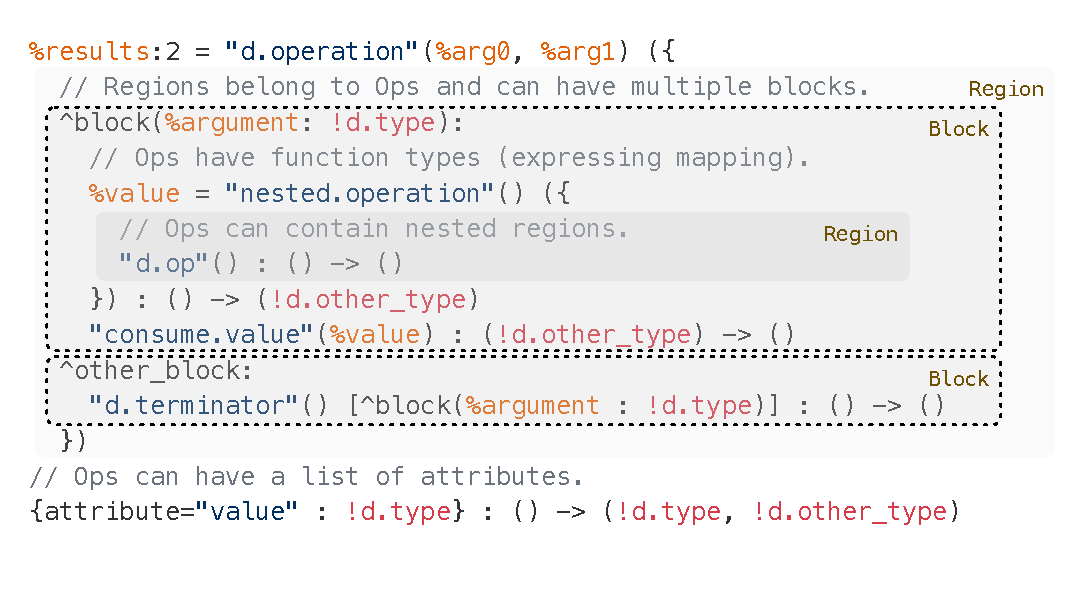
\includegraphics[width=.85\columnwidth]{img/structure_2.pdf}
  \caption{Operation (Op) is a main entity in \MLIR; operations contain a list
        of regions, regions contain a list of blocks, blocks contains a list of
        Ops, enabling recursive structures}
  \label{fig:structure}
\end{figure}

This section describes the design of the IR in \MLIR following the
principles from the previous section.

\begin{figure}[t]
  \centering
  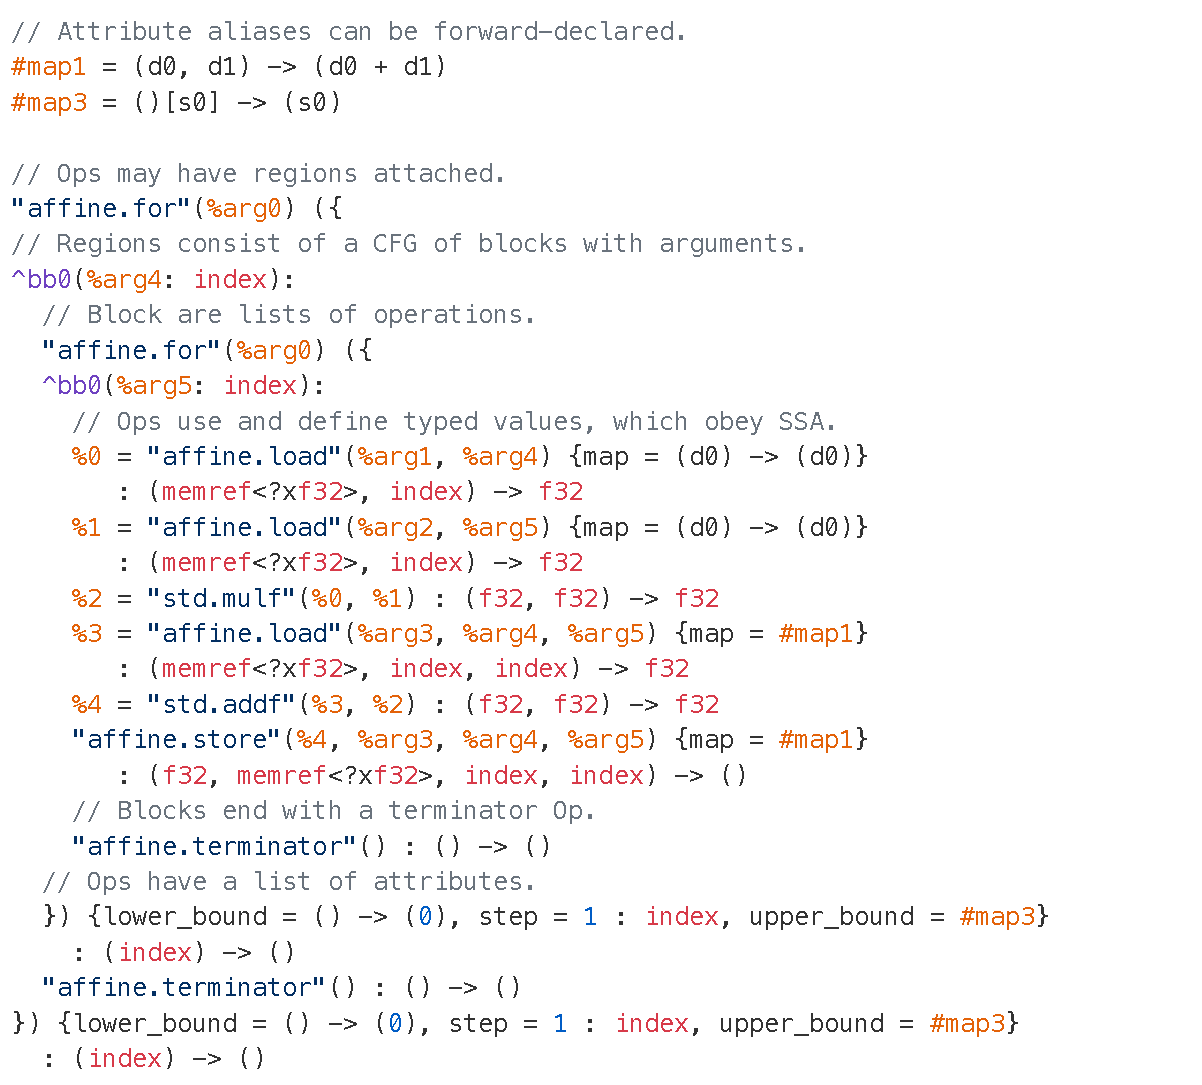
\includegraphics[width=.8\textwidth]{img/affine_generic_mlir.pdf}
  \caption{\MLIR \emph{generic} representation for polynomial multiplication
           using affine and std dialects. The same IR is displayed with the
           custom syntax~\figref{affine}.}
  \label{fig:generic}
\end{figure}

\paragraph{Operations}

The unit of semantics in \MLIR is an ``operation'', referred to as \emph{Op}.
Everything from ``instruction'' to ``function'' to ``module'' are modeled
as Ops in this system.  \MLIR does not have a fixed set of Ops, but
allows (and encourages) user-defined extensions---compiler passes
treat unknown Ops conservatively, and \MLIR has rich support for describing the
semantics of Ops to passes through traits, privileged operation hooks and
optimization interfaces as described in \secref{reusable_passes}.

Ops (see~\figref{structure}) have a unique opcode, which, textually, is a
string identifying its dialect and the operation.  Ops take and produce zero or more
\emph{values}, called \emph{operands} and \emph{results} respectively, and these
are maintained in SSA form. All values have a type, similarly to LLVM IR.
In addition to an opcode, operands and results, Ops
may also have \emph{Attributes}, \emph{Regions}, \emph{Block Arguments}, and
\emph{Location Information} as well. \figref{generic} illustrates values and Ops,
\lstinline|%|-identifiers are (packs of) named values, with ``\lstinline|:|''
specifying the number in a pack if more than one and ``\lstinline|#|'
a particular value. In the generic textual representation, operation names are
quoted string literals followed by operands in parentheses.

\paragraph{Attributes}

An \MLIR attribute is structured compile-time static
information, e.g., integer constant values, string data,
or a list of constant floating point values.  Attributes are typed, and each
Op instance has an open key-value dictionary from string names to attribute
values. In the generic syntax, attributes are between the Op
operands and its type as a brace-enclosed comma-separated list of key-value
pairs. For example, \figref{generic} uses attributes to define bounds
of a loop that are known to be constant affine forms:
\lstinline|{lower_bound = () -> (0), step = 1 : index,|
\lstinline| upper_bound = #map3}| where \lstinline|lower_bound|,
\lstinline|upper_bound| and \lstinline|step| are attribute names.
The \lstinline|() -> (0)| notation is used for inline affine forms, in this
case producing an affine function producing a constant \lstinline|0| value.
The \lstinline|#map3| notation is used for attribute \emph{aliases}, which
allow one to associate an attribute value with a label upfront and use the
label anywhere an attribute value is expected.

As with opcodes, there is no fixed set of attributes.  Attributes derive their
meaning either from the Op semantics or from the dialect (\secref{dialects}) they
are associated with.  Attributes are also extensible, allowing direct references
to foreign data structures, which is useful for integrating with existing systems.
For example, an attribute may refer to the contents of (known at compile time)
data storage in an ML system.

\paragraph{Location information}

\MLIR provides a compact representation for \emph{location information,}
and encourages the processing and propagation of this information
throughout the system.  It can be used to keep
the source program stack trace that produced an Op, to generate
debug information.  It standardizes the way to emit diagnostics from the compiler,
and is used by a wide range of testing tools.

Location information is also extensible, allowing a compiler to refer to
existing location tracking systems, high-level AST nodes, LLVM-style
file-line-column address, DWARF debugging info or whatever else is needed
for a high quality implementation.

\paragraph{Regions and blocks}

An instance of an Op may have a list of attached regions.  A \emph{region}
provides the mechanism for nested structure in \MLIR: a region contains a list
of blocks, and a block contains a list of operations (which may contain regions).
As with attributes, the semantics of a region are defined by the operation they
are attached to, however the blocks inside the region (if more than one) form a
Control Flow Graph (CFG).  For example, the \lstinline|affine.for| operation in
\figref{generic} is a loop with the single-block body attached as a region,
located between \lstinline|({| and \lstinline|})| delimiters.  The Op
specifies the flow of control across regions. In this example, the body is
executed repeatedly until the upper bound is reached.

The body of each region is a list of \emph{blocks}, and each block ends with a
\emph{terminator} operation, that may have \emph{successor} blocks to which the
control flow may be transferred. Each terminator
(e.g.\ ``switch'', ``conditional branch'' or ``unwind'') defines its
own semantics. It may chose to transfer the control flow to another block in
the same region, or return it to the Op enclosing the region. The graph of
successors defines a CFG, allowing standard SSA-based
control flow within a region.

Instead of using $\phi$ nodes, \MLIR uses a functional form of SSA~\cite{Appel98ssais}
where terminators pass values into \emph{block arguments} defined by the successor block.
Each block has a (potentially empty) list of typed block arguments, which are
regular values and obey SSA. The semantics of terminator Ops defines what
values the arguments of the block will take after the control is transferred.
For the first (entry) block of the region, the values are defined by the
semantics of the enclosing Op. For example, \lstinline|affine.for| uses the
entry block argument \lstinline|%arg4| as loop induction variable.

\paragraph{Value dominance and visibility}

Ops can only use values that are in scope, i.e. \emph{visible} according to
SSA dominance, nesting, and semantic restrictions imposed by enclosing
operations.  Values are visible within a CFG if they obey standard SSA
dominance relationships, where control is guaranteed to pass through a
definition before reaching a use.

Region-based visibility is defined based on simple nesting of regions:
if the operand to an Op is outside the current region, then it must be defined
lexically above and outside the region of the use.  This is what allows Ops
within an \lstinline|affine.for| operation to use values defined in outer scopes.

\MLIR also allows operations to be defined as \emph{isolated from above},
indicating that the operation
is a scope barrier---e.g.\ the ``std.func'' Op defines a function,
and it is not valid for operations within the function to refer to values
defined outside the function.  In addition to providing useful semantic
checking, a module containing isolated-from-above Ops may be processed
in parallel by an \MLIR compiler since no use-def chains may cross the
isolation barriers.  This is a important for compilation to utilize
multicore machines.

\paragraph{Symbols and symbol tables}

Ops can have a symbol table attached.  This table is a standardized way of
associating names, represented as strings, to IR objects, called \emph{symbols}. The
IR does not prescribe what symbols are used for, leaving it up to the Op
definition. Symbols are most useful for named entities need not obey SSA: they
cannot be redefined within the same table, but they can be used prior to their
definition. For example, global variables, functions or named modules can be
represented as symbols. Without this mechanism, it would have been impossible
to define, e.g., recursive function referring to themselves in their
definition. Symbol tables
can be nested if an Op with a symbol table attached has associated regions
containing similar Ops. \MLIR provides a mechanism to reference symbols from an
Op, including nested symbols.

\paragraph{Dialects}\label{sec:dialects}

\MLIR manages extensibility using \emph{Dialects}, which provide a logical
grouping of Ops, attributes and types under a unique namespace. Dialects
themselves do not introduce any new semantics but serve as a logical grouping
mechanism and can be used to provide dialect generic Op support (e.g.,
constant folding behavior for all ops in the dialect). The dialect namespace
appears as a dot-separated
prefix in the opcode, e.g., \figref{generic} uses \lstinline|affine| and
\lstinline|std| dialects.

The separation of Ops, types and attributes into dialects is conceptual
and is akin to designing a set of modular libraries. For example, a dialect can
contain Ops and types for operating on hardware vectors (e.g., shuffle,
insert/extract element, mask), and another dialect can contain Ops and types
for operating on algebraic vectors (e.g. absolute value, dot product, etc.).
Whether both dialects use the same vector type and where does this type belong
are design decisions left to the user of \MLIR.

While it is possible to put all Ops, types and attributes in a single dialect,
it would quickly become unmanageable due to the large number of simultaneously
present concepts and name conflicts, amongst other issues.
Although each Op, type and attribute belongs to exactly one dialect, \MLIR
explicitly supports a mix of dialects to enable progressive lowering. Ops from
different dialects can coexist at any level of the IR at any time, they can use
types defined in different dialects, etc. Intermixing of dialects allows for
greater reuse, extensibility and provides flexibility that otherwise would
require developers to resort to all kinds of non-composable workarounds.

\paragraph{Type system}

Each value in \MLIR has a type, which is specified in the Op
that produces the value or in the block that defines the value as an argument.
Types provide compile-time semantics for the IR. The type system in \MLIR is
user-extensible, and may refer to existing foreign type systems (e.g. an
\lstinline|llvm::Type| or a \lstinline|clang::Type|). \MLIR enforces strict type
equality checking and does not provide type conversion rules. Ops list their
inputs and result types using trailing function-like syntax. In \figref{generic},
\lstinline|std.load| maps from the memory reference and
index types to the type of the value it loads.

From the type theory point of view, \MLIR only supports non-dependent types,
including trivial, parametric, function, sum and product types. While it is
possible to implement a dependent type system by combining Ops with
symbols and user-defined types in a literal interpretation of Curry-Howard
isomorphism, such types will be opaque to the IR.

\paragraph{Standard types}

In addition, \MLIR provides a standardized set of commonly used types,
including arbitrary precision integers, standard floating point types, and simple
common containers---tuples, multi-dimensional vectors, and tensors.  These types
are merely a convenience that are useful to authors of dialects, but their use is not
required.

\paragraph{Functions and modules}

Similarly to conventional IRs, \MLIR is usually structured into functions and
modules.  However, these are not new or separate concepts in \MLIR: they are
implemented as Ops in the builtin dialect.

A module is an Op with a single region containing a single block, and
terminated by a dummy Op that does not transfer the control flow. A module defines a
symbol and can be referenced. Like any block, its body contains a list of Ops,
which may be functions, global variables, compiler metadata, or other top-level
constructs.

A function is an Op with a single region, with arguments corresponding to
function arguments. It defines a symbol and can be referenced by name. The
control flow is transferred into a function using a function call Op. Once
inside, the control flow follows the CFG of the blocks in the region. A
``return'' terminator does not have successors and instead terminates the
region execution, transferring the control flow back to the call-site of the
function.
Any operands of the ``return'' terminator Op are the returned values of the
function.
